\begin{figure}[h]
\centering
\caption{Materiais e robô após montagem}
\label{fig:RoboReal}
	\begin{subfigure}[b]{0.49\textwidth}%
		\centering
		% fbox{}
		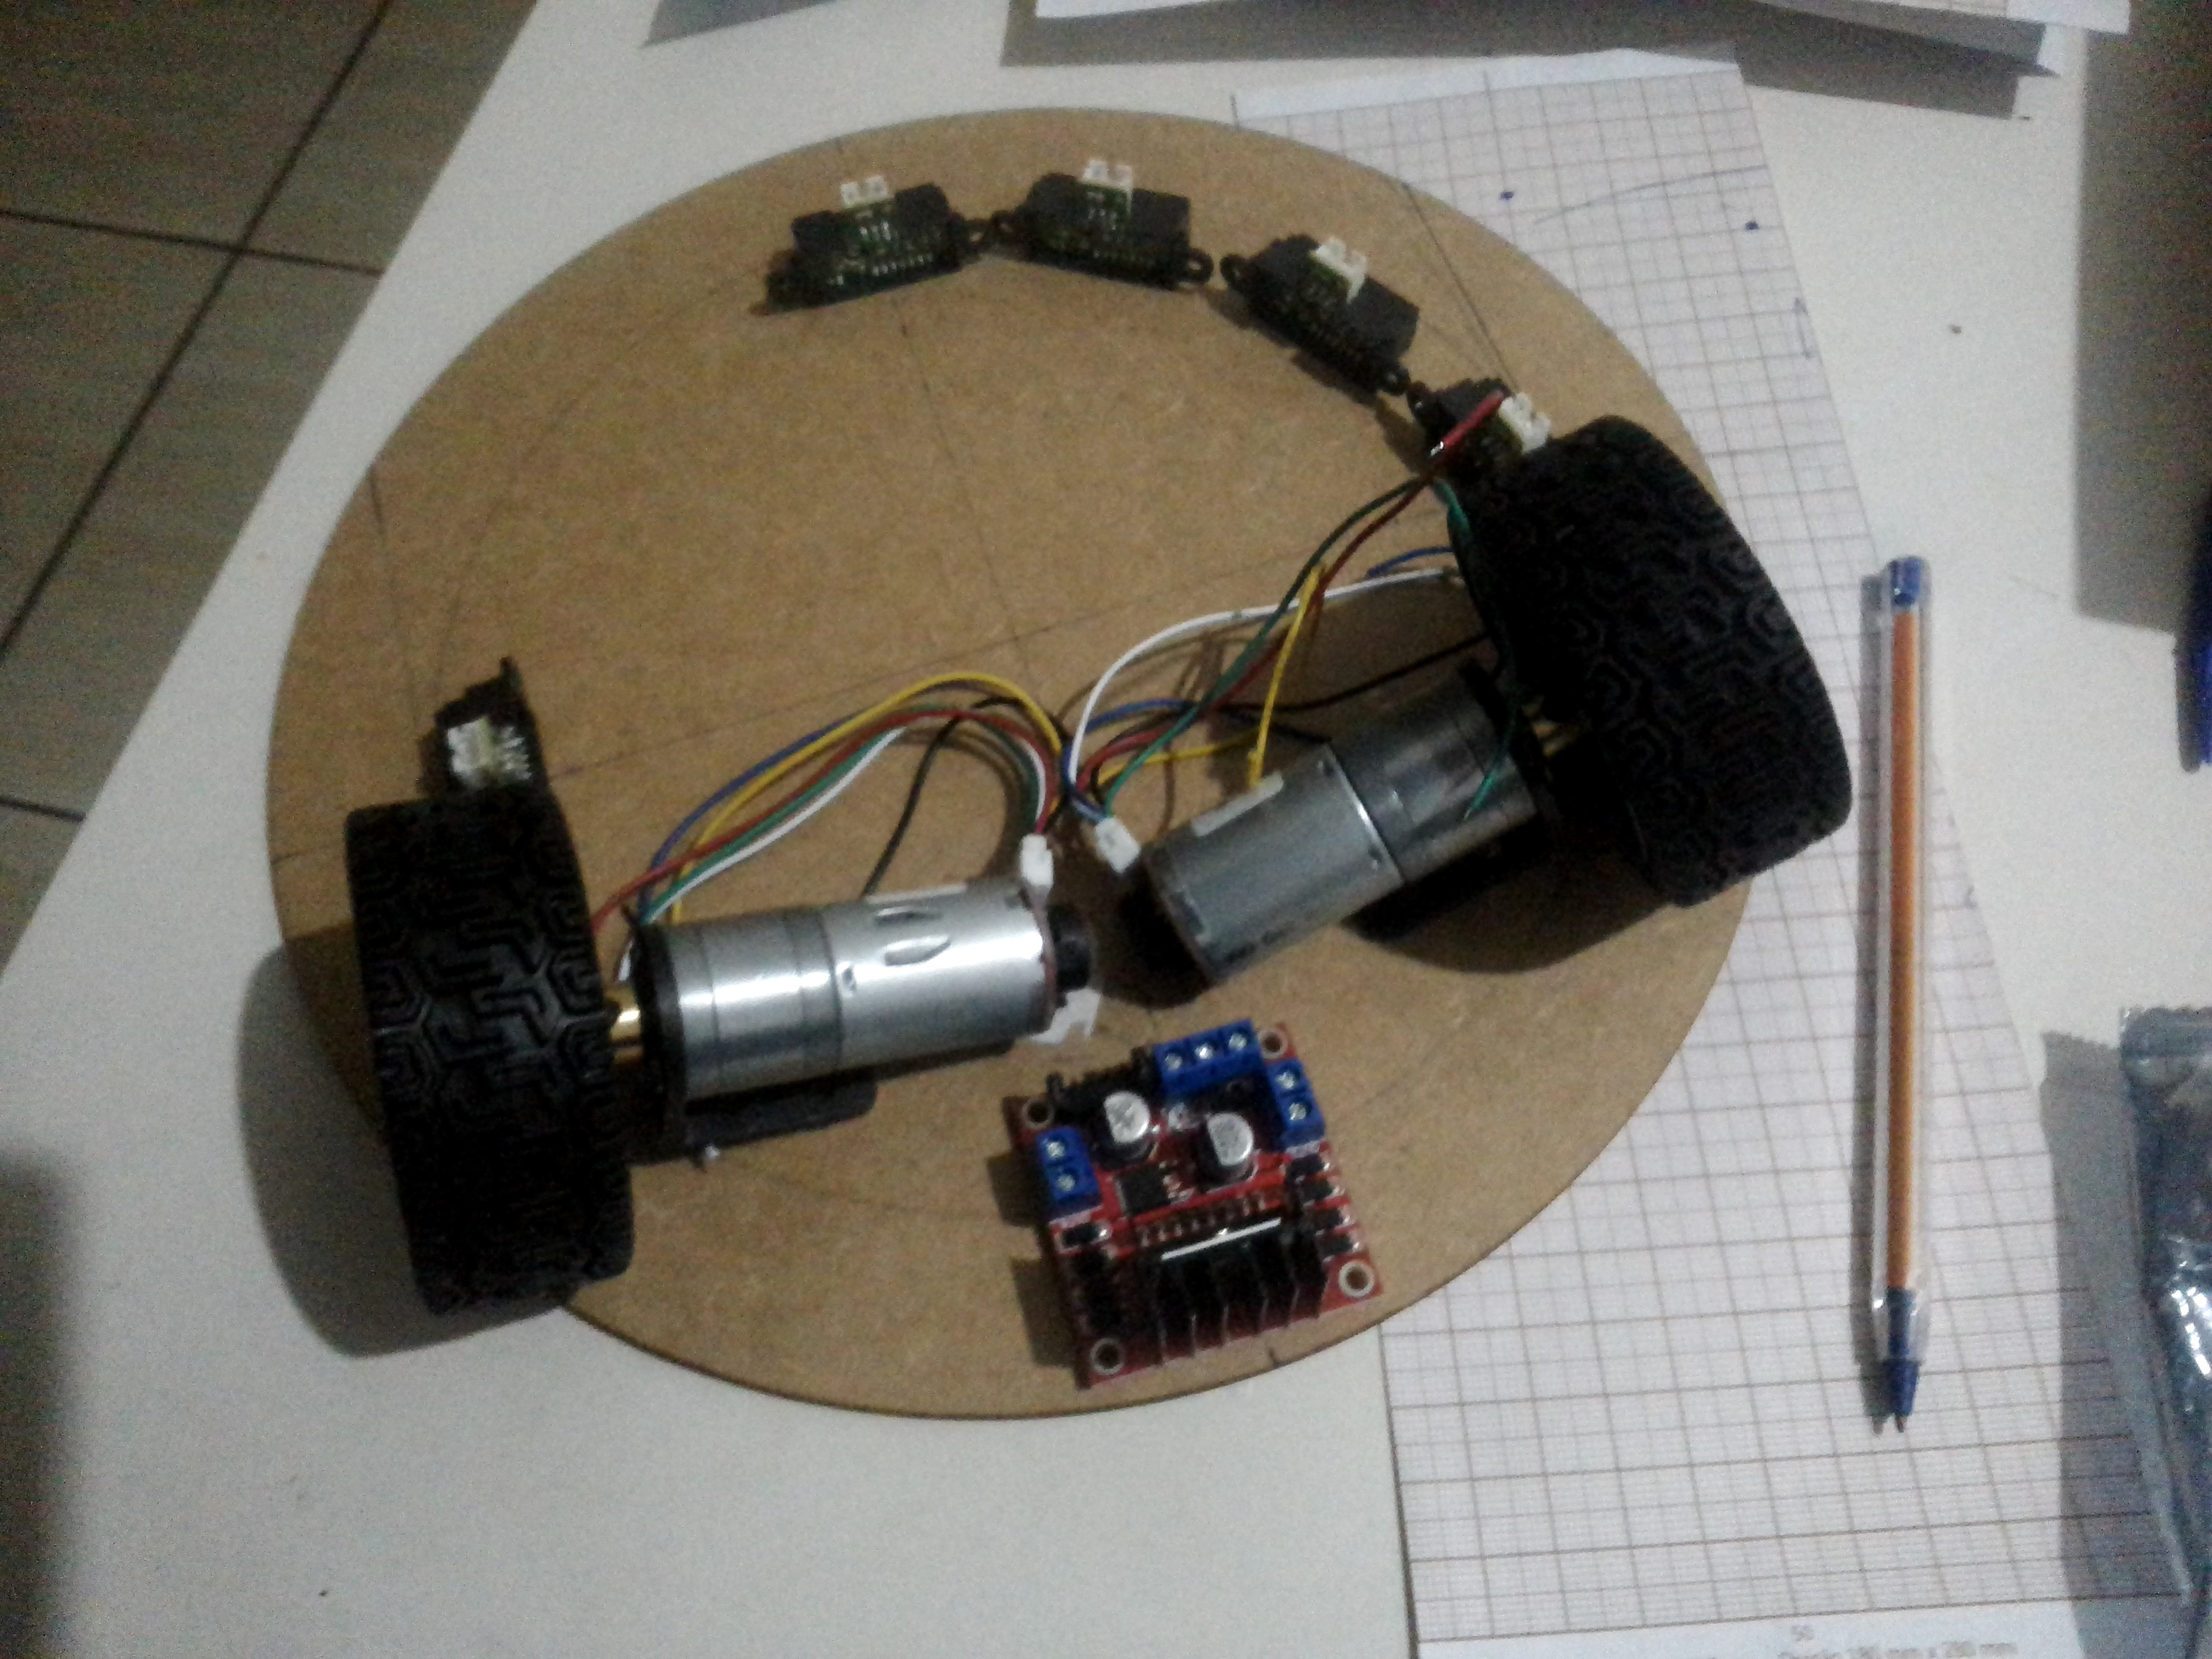
\includegraphics[trim= 0cm 0cm 0cm 0cm,clip,
scale=0.07]{Figuras/Robo1}
		\subcaption{Materiais do robô}
	  	%\label{fig:test1}
	\end{subfigure}
	~
	\begin{subfigure}[b]{0.49\textwidth}%
		\centering
		% fbox{}
		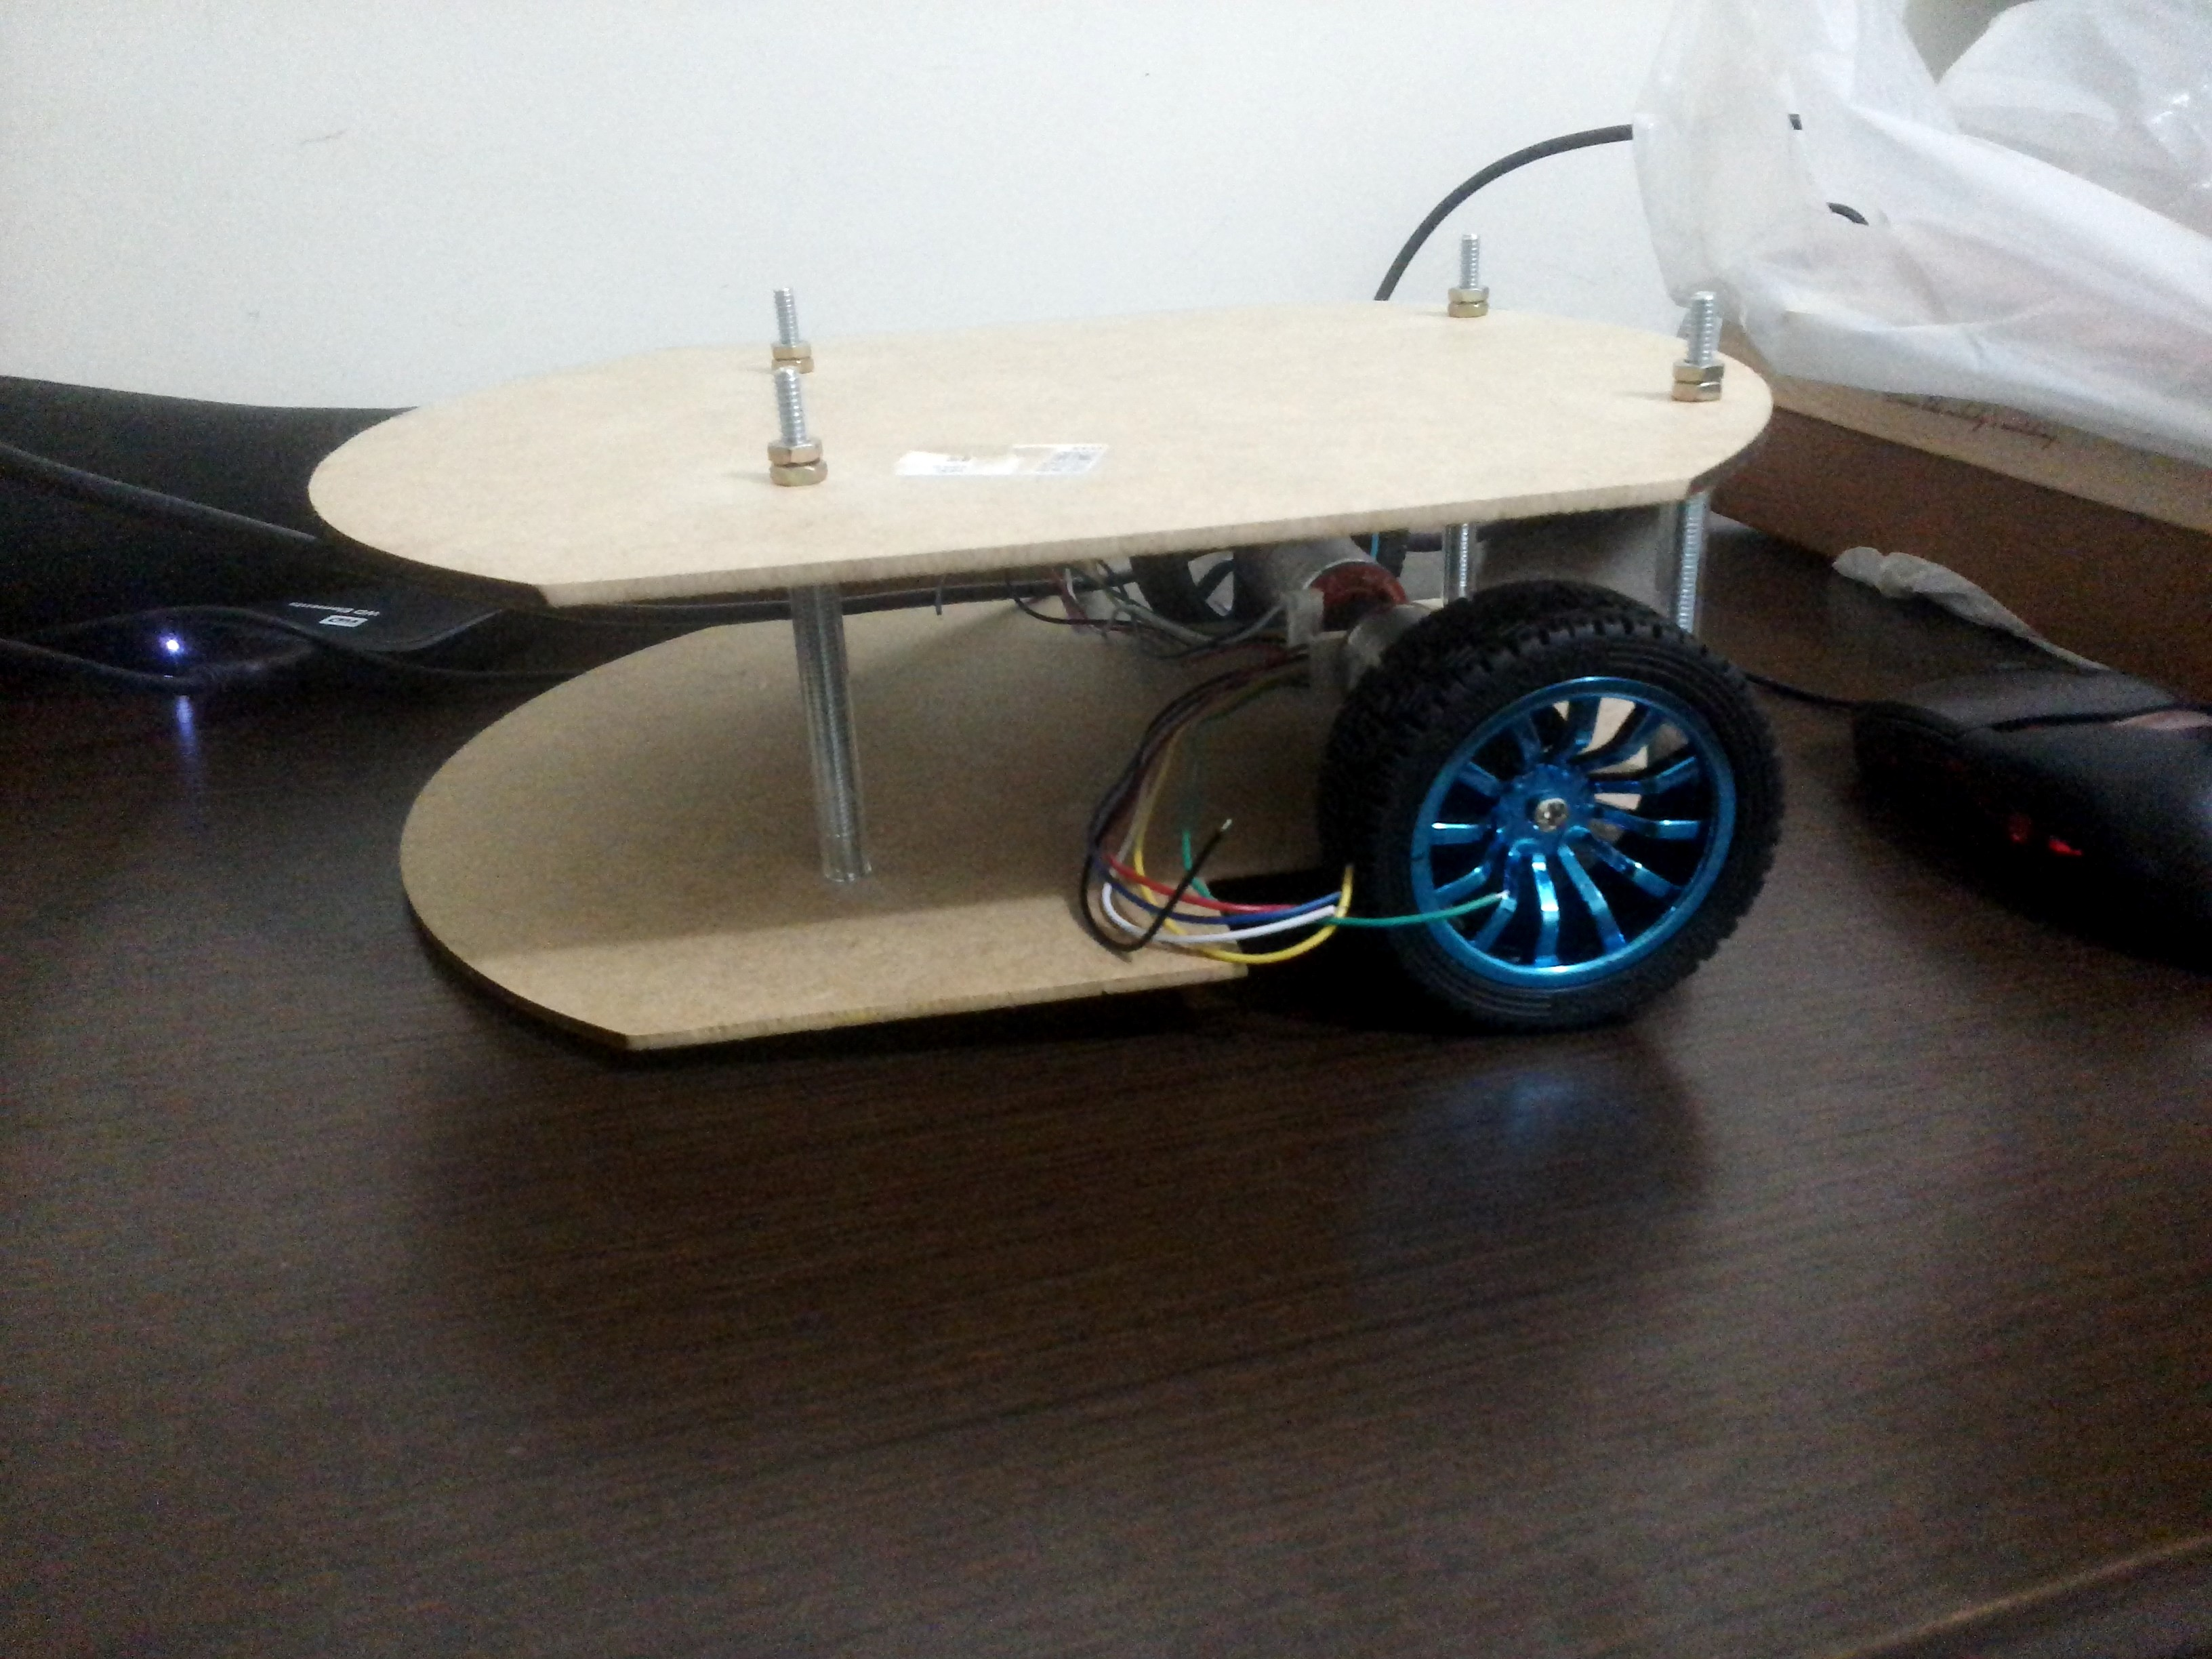
\includegraphics[trim={0cm 0cm 0cm 0cm},clip,
scale=0.07]{Figuras/Robo2}
		\subcaption{Robô montado}
	  	%\label{fig:test2}
	\end{subfigure}
	
	\textbf{Fonte: autoria própria}
\end{figure}